\documentclass[../SimBALink.tex]{subfiles}
\begin{document}

\subsection{Tires}
\begin{gather}
\notag \textbf{Rolling Resistance} \\
K_t = 
\left\{
  \begin{array}{lr}
    0.0085 + \frac{0.18}{p_t} + \frac{1.59*10^{-6}}{p_t} & : v_{kph} \le 165 (km/h)\\
    \frac{0.18}{p_t} + \frac{2.91*10^{-6}}{p_t} & : v_{kph} > 165 (km/h)
  \end{array}
\right. \\
\notag \textbf{Wheel Slip} \\
\kappa = \frac{v - \omega_t r_t}{v} \\
\mu_{t,gnd} = D_{\kappa}\sin(C_{\kappa} \arctan[B_{\kappa}\kappa - E_{\kappa}(B_{\kappa}\kappa - \arctan B_{\kappa}\kappa)]) \\
\notag \textbf{Load and Torque} \\
\tau_t = \tau_g - \frac{F_{w,long}}{r_t} - \frac{F_b}{r_b} - K_t F_{w,n} v_{kph}^2 \\
\notag \textbf{Traction Limiting} \\
F_{max} = \mu_{t,gnd} F_{w,n} \\
F = \tau r_t \\
F_t =
\left\{
  \begin{array}{lr}
	F & : -F_{max} \le F \le F_{max} \\
	F_{max} & : -F_{max} > F > F_{max}
  \end{array}
\right. 
\end{gather}

The tire coefficient ($\mu_{t,gnd}$) is modeled using the "Magic Formula" as shown below. Where $D_{\kappa}$ is the maximum tire coefficient of the tire.

 \begin{figure}[h!]
  \centering
  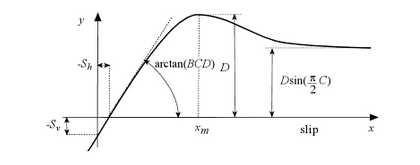
\includegraphics[scale=1]{magic_formula}
  \caption{Magic Formula }
\end{figure}

\end{document}